% C2GES original-title reconstruction, Round 1.
% All domain results come from frozen offline protocol v0.2 and its reproduction.
\documentclass[applsci,article,submit,moreauthors]{Definitions/mdpi}
\firstpage{1}
\makeatletter\setcounter{page}{\@firstpage}\makeatother
\pubvolume{1}\issuenum{1}\articlenumber{0}\pubyear{2026}\copyrightyear{2026}
\datereceived{}\daterevised{}\dateaccepted{}\datepublished{}
\newcommand{\cges}{C\textsuperscript{2}GES}
\setlength{\headheight}{20pt}
\AtBeginDocument{\pdfstringdefDisableCommands{\def\cges{C2GES}}}

\Title{Causal and Counterfactual Graph-Enhanced Extractive Summarization (C\textsuperscript{2}GES) for Power Grid Maintenance Reports}
\Author{Liu Bijing $^{1,2}$ and Yang Yong $^{1,2,}$*}
\AuthorNames{Liu Bijing and Yang Yong}
\address{$^{1}$ \quad NARI Group Corporation (State Grid Electric Power Research Institute), Nanjing 211106, Jiangsu Province, China;\\
$^{2}$ \quad Beijing Kedong Electric Power Control System Co., Ltd., Beijing 100080, China}
\corres{Correspondence: Yang Yong; email address to be provided before submission}

\abstract{Power-grid reliability reports contain event descriptions, causes, propagation paths, impacts, and mitigation actions that are difficult to retain in a short extractive summary. We present \cges{}, an offline causal- and counterfactual-graph-enhanced extractive method. The implemented system assigns sentence-level causal-role scores, constructs a typed directed proxy graph, measures deterministic counterfactual sensitivity as the loss of graph flow after removing a sentence node, and selects sentences under length, causal-function coverage, redundancy, and source-order constraints. A benchmark was constructed from 40 public North American Electric Reliability Corporation reports. Twenty-eight reports with extractable official Executive Summaries were retained and split by document hash into 12 development and 16 test reports. Seven methods were evaluated on identical candidates at five- and ten-sentence budgets. At five sentences, full \cges{} obtained ROUGE-1/2/L F1 of 0.2608/0.0934/0.1323. Its ROUGE-1 difference was +0.0388 over Lead (95\% report-level bootstrap interval [0.0141, 0.0663]) and +0.0390 over TextRank ([0.0060, 0.0786]). Centroid nevertheless had the highest observed ROUGE-L at both budgets. A strict counterfactual ablation was tied with Full at five sentences; at ten sentences, Full was lower by 0.0160 ROUGE-1, with unadjusted interval [-0.0320,-0.0005]. Thus, the experiment does not support a counterfactual-component benefit or broad superiority. A local MiniLM semantic-centroid baseline was statistically unresolved relative to Full. Two independent executions produced byte-identical predictions, aggregate metrics, and bootstrap outputs. The study supplies an auditable domain benchmark and deterministic method baseline while leaving development-only counterfactual redesign and expert validation to future work.}
\keyword{extractive summarization; causal event graph; counterfactual intervention; power-grid reliability reports; NERC; reproducible evaluation}
\featuredapplication{The framework produces a length-constrained, source-traceable extract from a power-grid reliability report while exposing sentence identifiers, proxy-graph relations, and structural intervention scores. It is decision support and requires engineering review before consequential use.}

\begin{document}

\section{Introduction}

Power-grid disturbance, maintenance, and lessons-learned reports record more than isolated facts. Engineers often need the sequence connecting a condition or root cause to an initiating event, propagation or system response, operational impact, and corrective action. A short summary that preserves equipment names and quantities while breaking those connections may remain lexically relevant but provide little support for root-cause review. Extractive summarization is attractive in this setting because every selected sentence can retain a stable identifier and a direct link to the official report.

Evidence selection and query-focused summarization provide foundations for this task. FEVER established sentence-level evidence retrieval as an independently assessable problem \cite{thorne2018fever}; query-focused summarization conditions selection on an information need rather than only global topical salience \cite{zhong2021qmsum,vig2022exploring,zhong2020extractive}. Graph-based extractive systems model structural relations between sentences or discourse units \cite{wang2020heterogeneous,cui2020enhancing,jing2021multiplex}. Causal NLP asks a different question: whether textual relations support directional or intervention-relevant interpretation rather than association alone \cite{feder2022causal,du2022ecare}.

The original \cges{} concept proposed a broader neural architecture and a manually annotated power-grid corpus. Those claims are not retained because the audited assets do not contain the claimed GNN/T5 implementation, expert adjudication, or reported GridMaint-CausalSum results. The present article retains the application question and original title while grounding its method in executable offline code, public source reports, frozen configurations, complete prediction ledgers, and independently reproduced output hashes. The implemented graph is a deterministic causal proxy graph, not a trained GNN or a structural model of grid physics.

Public North American Electric Reliability Corporation (NERC) reports supply authentic technical language and report structure \cite{nercEventAnalysis,nerc2015qualityreport}. The official Executive Summary is used as the summary reference. Existing five-role evidence records are machine-verified silver candidates used for graph construction and a diagnostic coverage measure; they are not human or domain-expert gold. This distinction prevents machine agreement from being treated as independent causal validation.

The article makes four scoped contributions. First, it creates a hash-defined report-level benchmark that records all inclusion and exclusion decisions. Second, it implements a typed sentence graph, deterministic node/edge intervention, graph-flow sensitivity, and a constrained extractive selector. Third, it evaluates Lead, lexical and semantic centroids, TextRank, Role, strict no-counterfactual, and full \cges{} conditions at two budgets with report-level paired bootstrap intervals. Fourth, it reports the negative counterfactual result and exact reproduction rather than asserting component effectiveness or state-of-the-art performance.

\section{Related Work}

\subsection{Extractive and Query-Focused Summarization}

Extractive summarization selects source sentences instead of generating new text, preserving traceability. Matching-based methods, iterative ranking, and unsupervised graph objectives offer transparent baselines \cite{zhong2020extractive,bi2021aredsum,liu2021unsupervised}. Query-focused benchmarks further show that the same document can require different extracts under different information needs \cite{zhong2021qmsum,vig2022exploring}. The present benchmark is global report summarization rather than open-corpus retrieval: each method receives the same candidate sentences from one report and returns a fixed-size extract.

\subsection{Evidence Retrieval and Semantic Ranking}

Fact verification evaluates sentence evidence retrieval separately from claim classification \cite{thorne2018fever}. BM25 and dense sentence encoders are strong evidence-ranking comparators \cite{robertson2009probabilistic,reimers2019sentencebert}. The existing \cges{} asset base includes a separate document-grouped FEVER study. That study verifies an auditable ranking implementation but is not a power-grid summarization result. The present domain run adds a local, hash-bound all-MiniLM-L6-v2 semantic-centroid baseline without network access.

\subsection{Graph Structure and Causal NLP}

Graph summarizers connect sentences, entities, topics, or discourse units before ranking or message passing \cite{wang2020heterogeneous,cui2020enhancing,jing2021multiplex}. The implemented \cges{} graph is simpler: dominant sentence roles permit typed transitions, and weighted degree supplies graph salience. It sacrifices learned capacity for transparent construction and deterministic intervention.

Causal NLP includes relation extraction, inference over text-derived variables, robustness analysis, and counterfactual data construction \cite{feder2022causal,du2022ecare}. Counterfactual is used narrowly here. Removing a graph node and its incident edges measures how much registered graph flow depends on that sentence. It neither generates altered event text nor estimates a physical causal effect.

\subsection{Power-Grid Technical Text}

AI and language technologies are increasingly considered for grid models, operational records, and infrastructure analysis \cite{xie2022massively,hamann2024foundation,madabhushi2023survey,srinivasan2023artificial}. Verified power-grid NLP work includes supervised entity--relation extraction from a purpose-built grid-field corpus \cite{meng2023gridfield}. That task differs from report-level extractive summarization. We do not claim superior relation extraction or validated physical causality.

\section{Materials and Methods}

\subsection{Task and Source Reports}

Let a report be a candidate sentence sequence $D=\{s_1,\ldots,s_n\}$ with stable identifiers and positions. Given budget $K$, a method returns $\hat{Y}_K\subseteq D$, where $|\hat{Y}_K|=\min(K,n)$. Selected sentences are restored to source order. The official Executive Summary is the reference, and the frozen budgets are $K\in\{5,10\}$.

The registered source contains 40 public NERC PDFs spanning disturbances, reliability reviews, storms, recommendations, and technical assessments. Thus, ``maintenance reports'' in the retained title denotes the intended engineering-review use; the measured corpus is described precisely as public NERC reliability and disturbance reports. Layout-preserving PDF text is eligible when an Executive Summary and deterministic end boundary can be identified and the cleaned summary has at least 80 words. Candidate sentences come from the segmented body after removal of the detected summary prefix.

An initial build incorrectly extended one Executive Summary to 25,209 words because the report transitioned to a Chapter~1 heading not covered by the earlier rule. That output directory was retained as a failed diagnostic and excluded. A Chapter~1 boundary rule and regression test were added before a new build. The corrected frozen dataset contains 28 reports: 12 development and 16 test reports, with 12 exclusions recorded by reason. Test references contain 279--2298 words (median 790.5), while candidate pools contain 20--60 sentences (median 54). Document IDs are assigned by SHA-256 buckets, and no report crosses partitions. The dataset SHA-256 is \texttt{3B74CA2E...25A7C48}.

\subsection{Silver Role Boundary}

Optional candidate evidence represents trigger event, root cause, propagation or response, impact, and mitigation. These records were produced and checked by machine workflows. They are silver development signals, not independent expert annotations. A supplied silver role can resolve a lexical tie during graph construction. Silver role coverage is the fraction of roles with available evidence for which at least one registered sentence is selected. Because the same layer can influence selection, this measure is diagnostic internal consistency and not expert causal fidelity.

\subsection{Sentence Roles and Typed Proxy Graph}

For sentence $s_i$ and role $r$, a transparent cue function counts registered phrases. Longer phrases receive a small additional weight, and engineering quantities such as MW, GW, kV, Hz, and percentages contribute an impact cue. Non-negative scores are divided by the document maximum for each role. The dominant role is the highest score, with explicit silver evidence taking precedence over lexical ties.

Each sentence becomes a graph node. Directed edges are permitted for root-cause $\rightarrow$ trigger, root-cause $\rightarrow$ propagation, trigger $\rightarrow$ propagation, trigger/propagation $\rightarrow$ impact, impact $\rightarrow$ mitigation, and root-cause $\rightarrow$ mitigation transitions. For an allowed pair within 12 positions,
\begin{equation}
w_{ij}=0.45\exp(-d_{ij}/5)+0.30J(s_i,s_j)+0.25\min(R_i,R_j),
\end{equation}
where $d_{ij}$ is absolute sentence distance, $J$ is token-set Jaccard similarity, and $R_i,R_j$ are dominant-role scores. Direction follows role semantics rather than narrative order. Graph salience $G_i$ is normalized weighted degree. These edges are textual proxies and have not been validated as physical causal relations.

Figure~\ref{fig:implemented-architecture} shows the implemented offline pipeline and its actual data dependencies. The graph is a deterministic sentence-level proxy graph, not a learned GNN; the intervention removes a node and its incident edges, rather than generating synthetic counterfactual text; and neither graph construction nor inference invokes an external model API. The optional silver evidence is machine-produced and is not human or expert gold.

\begin{figure}[H]
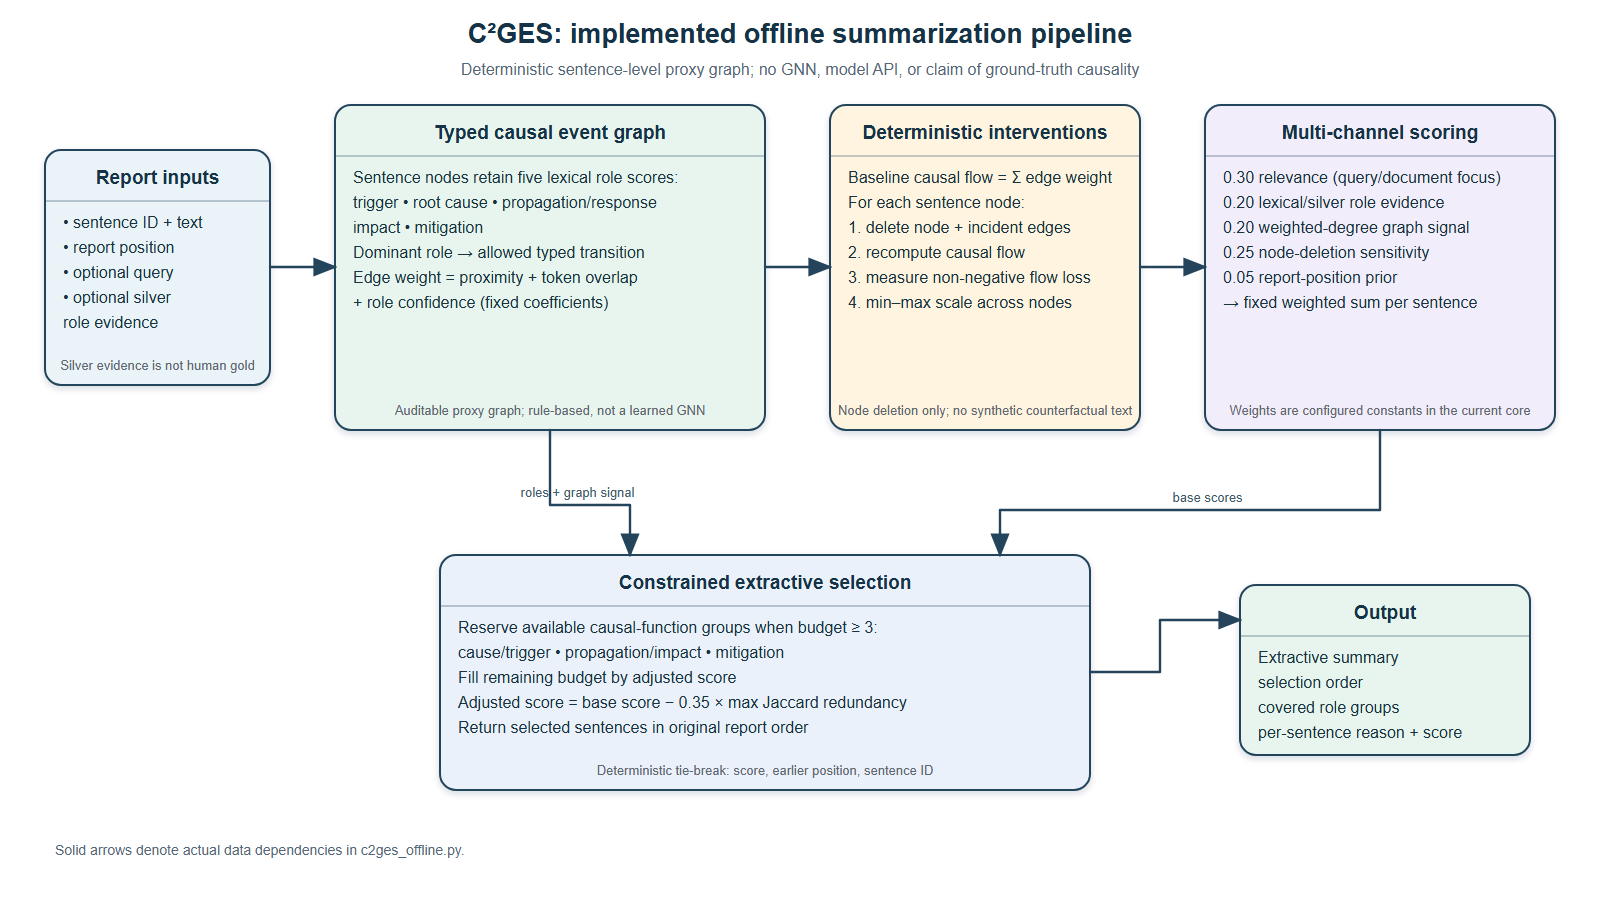
\includegraphics[width=\textwidth]{figures/fig_c2ges_implemented_architecture_r1_qa2.png}
\caption{Implemented C\textsuperscript{2}GES offline architecture in protocol v0.2. Solid arrows denote executable data dependencies. The displayed weights are the frozen Full-condition coefficients; the graph and node-deletion intervention are auditable textual proxies and do not constitute a GNN, a physical simulator, or ground-truth causal identification.}
\label{fig:implemented-architecture}
\end{figure}

\subsection{Deterministic Graph Intervention}

Total typed graph flow is
\begin{equation}
F(G)=\sum_{e\in E(G)} w_e.
\end{equation}
For each node $i$, a new graph $G_{-i}$ removes the node and all incident edges. Counterfactual sensitivity is
\begin{equation}
C_i=\operatorname{norm}\left(\max\{0,F(G)-F(G_{-i})\}\right).
\end{equation}
The original graph remains immutable, and unknown interventions fail closed. This leave-one-node-out quantity measures proxy-graph dependence, not a Pearl-style intervention on an identified physical system.

\subsection{Scoring and Constrained Selection}

Full \cges{} scores sentence $i$ as
\begin{equation}
S_i=0.30Q_i+0.20R_i+0.20G_i+0.25C_i+0.05P_i,
\end{equation}
where $Q_i$ is offline document-centroid relevance, $R_i$ is role compatibility, $G_i$ is graph salience, $C_i$ is graph-intervention sensitivity, and $P_i=1/(1+\mathrm{position}_i)$. These are frozen defaults, not test-tuned weights.

When $K\geq3$, selection reserves one sentence for each available group: cause/trigger, propagation/impact, and mitigation. Remaining slots maximize
\begin{equation}
S_i-0.35\max_{j\in A}J(s_i,s_j),
\end{equation}
where $A$ contains already selected sentences. Ties prefer earlier position and then sentence ID. The final extract returns to source order.

\subsection{Conditions and Strict Counterfactual Ablation}

Seven conditions share reports, candidates, and budgets: Lead; lexical Centroid; TextRank using NetworkX PageRank; Semantic Centroid using a local all-MiniLM-L6-v2 snapshot; Role-only ranking; Graph without CF; and Full. The strict no-CF condition removes only the 0.25 counterfactual channel. Dividing the retained Full weights by 0.75 yields 0.40 relevance, 0.2667 role, 0.2667 graph, 0.0667 position, and zero CF. The redundancy penalty and all other decisions are unchanged.

\subsection{Frozen Evaluation and Statistics}

Protocol v0.2 fixes both budgets, condition order, 10,000 bootstrap samples, the semantic-model revision, runtime, model-tree hash, and report as resampling unit. Python 3.12.10, NetworkX 3.6.1, sentence-transformers 5.6.0, CPU PyTorch 2.13.0, and rouge-score 0.1.2 were used. The runner refuses an existing output directory and verifies configuration, data, code, runtime, and model hashes before prediction.

ROUGE-1, ROUGE-2, and ROUGE-L F1 compare extracts with the official summary. ROUGE-L is primary. Mean pairwise Jaccard measures redundancy. For every baseline and ROUGE metric, paired report-level bootstrap resamples the 16 reports 10,000 times and records Full minus baseline. The emitted $p$ values are exploratory and unadjusted across the comparison family; interpretation therefore emphasizes effects and intervals \cite{cameron2008bootstrap}.

\section{Results}

\subsection{Five-Sentence Results}

Table~\ref{tab:k5} reports $K=5$. Full \cges{} obtains ROUGE-1/2/L F1 of 0.2608/0.0934/0.1323. Centroid has the highest observed ROUGE-2 and ROUGE-L, and strict no-CF has the highest observed ROUGE-1. Full has lower redundancy than lexical Centroid, TextRank, and Semantic Centroid, but Lead has the lowest redundancy. Silver coverage is highest for Role and remains a machine-label diagnostic.

\begin{table}[H]
\caption{Frozen NERC report summarization at $K=5$. Bold marks the observed column maximum only.}
\label{tab:k5}
\centering
\begin{tabular}{lrrrrr}
\toprule
Condition & R-1 F1 & R-2 F1 & R-L F1 & Silver coverage & Redundancy\\
\midrule
Lead & 0.2220 & 0.0876 & 0.1262 & 0.2125 & \textbf{0.0539}\\
Centroid & 0.2564 & \textbf{0.1002} & \textbf{0.1405} & 0.2500 & 0.1645\\
TextRank & 0.2218 & 0.0822 & 0.1267 & 0.1625 & 0.1845\\
Semantic Centroid & 0.2483 & 0.0889 & 0.1270 & 0.2125 & 0.1031\\
Role & 0.2367 & 0.0831 & 0.1185 & \textbf{0.4250} & 0.0614\\
Graph without CF (strict) & \textbf{0.2616} & 0.0924 & 0.1320 & 0.3875 & 0.0805\\
\cges{} Full & 0.2608 & 0.0934 & 0.1323 & 0.3750 & 0.0683\\
\bottomrule
\end{tabular}
\end{table}

Full minus Lead is +0.0388 on ROUGE-1, with 95\% percentile interval [0.0141, 0.0663]. Full minus TextRank is +0.0390, with interval [0.0060, 0.0786]. Their ROUGE-2 and ROUGE-L intervals cross zero. Full minus Semantic Centroid is +0.0125/+0.0045/+0.0052 on ROUGE-1/2/L, with all intervals crossing zero. Full minus Centroid ROUGE-L is -0.0082, interval [-0.0255, 0.0058]. Thus, the only v0.2 five-sentence ROUGE intervals excluding zero are the Full ROUGE-1 contrasts with Lead and TextRank.

\subsection{Strict Counterfactual Ablation}

At $K=5$, Full minus strict no-CF is -0.0009 for ROUGE-1 (interval [-0.0089, 0.0061]), +0.0010 for ROUGE-2 ([-0.0064, 0.0085]), and +0.0003 for ROUGE-L ([-0.0048, 0.0060]). The ablation therefore provides no evidence that graph-flow counterfactual sensitivity improves five-sentence overlap.

At $K=10$, Full minus strict no-CF is -0.0160 for ROUGE-1, with unadjusted interval [-0.0320, -0.0005]. ROUGE-2 and ROUGE-L differences are -0.0120 and -0.0075, with intervals crossing zero. This pattern is unfavorable to the current CF score: it supplies no benefit at $K=5$ and has a wholly negative exploratory ROUGE-1 interval at $K=10$. Because the family is not multiplicity-adjusted, we do not generalize this observation beyond the frozen benchmark.

\subsection{Ten-Sentence Sensitivity}

Table~\ref{tab:k10} shows higher overlap for all methods at $K=10$, as expected when longer extracts are compared with long references. Strict no-CF has the highest observed ROUGE-1 and ROUGE-2; Centroid retains the highest observed ROUGE-L. Full has no supported difference from Semantic Centroid.

Figure~\ref{fig:rouge-budgets} visualizes the same frozen aggregate ROUGE values in Tables~\ref{tab:k5} and~\ref{tab:k10}; it is descriptive and adds no new statistical test. In particular, the figure makes visible that the strict no-CF condition is at least competitive with Full at both budgets.

\begin{figure}[H]
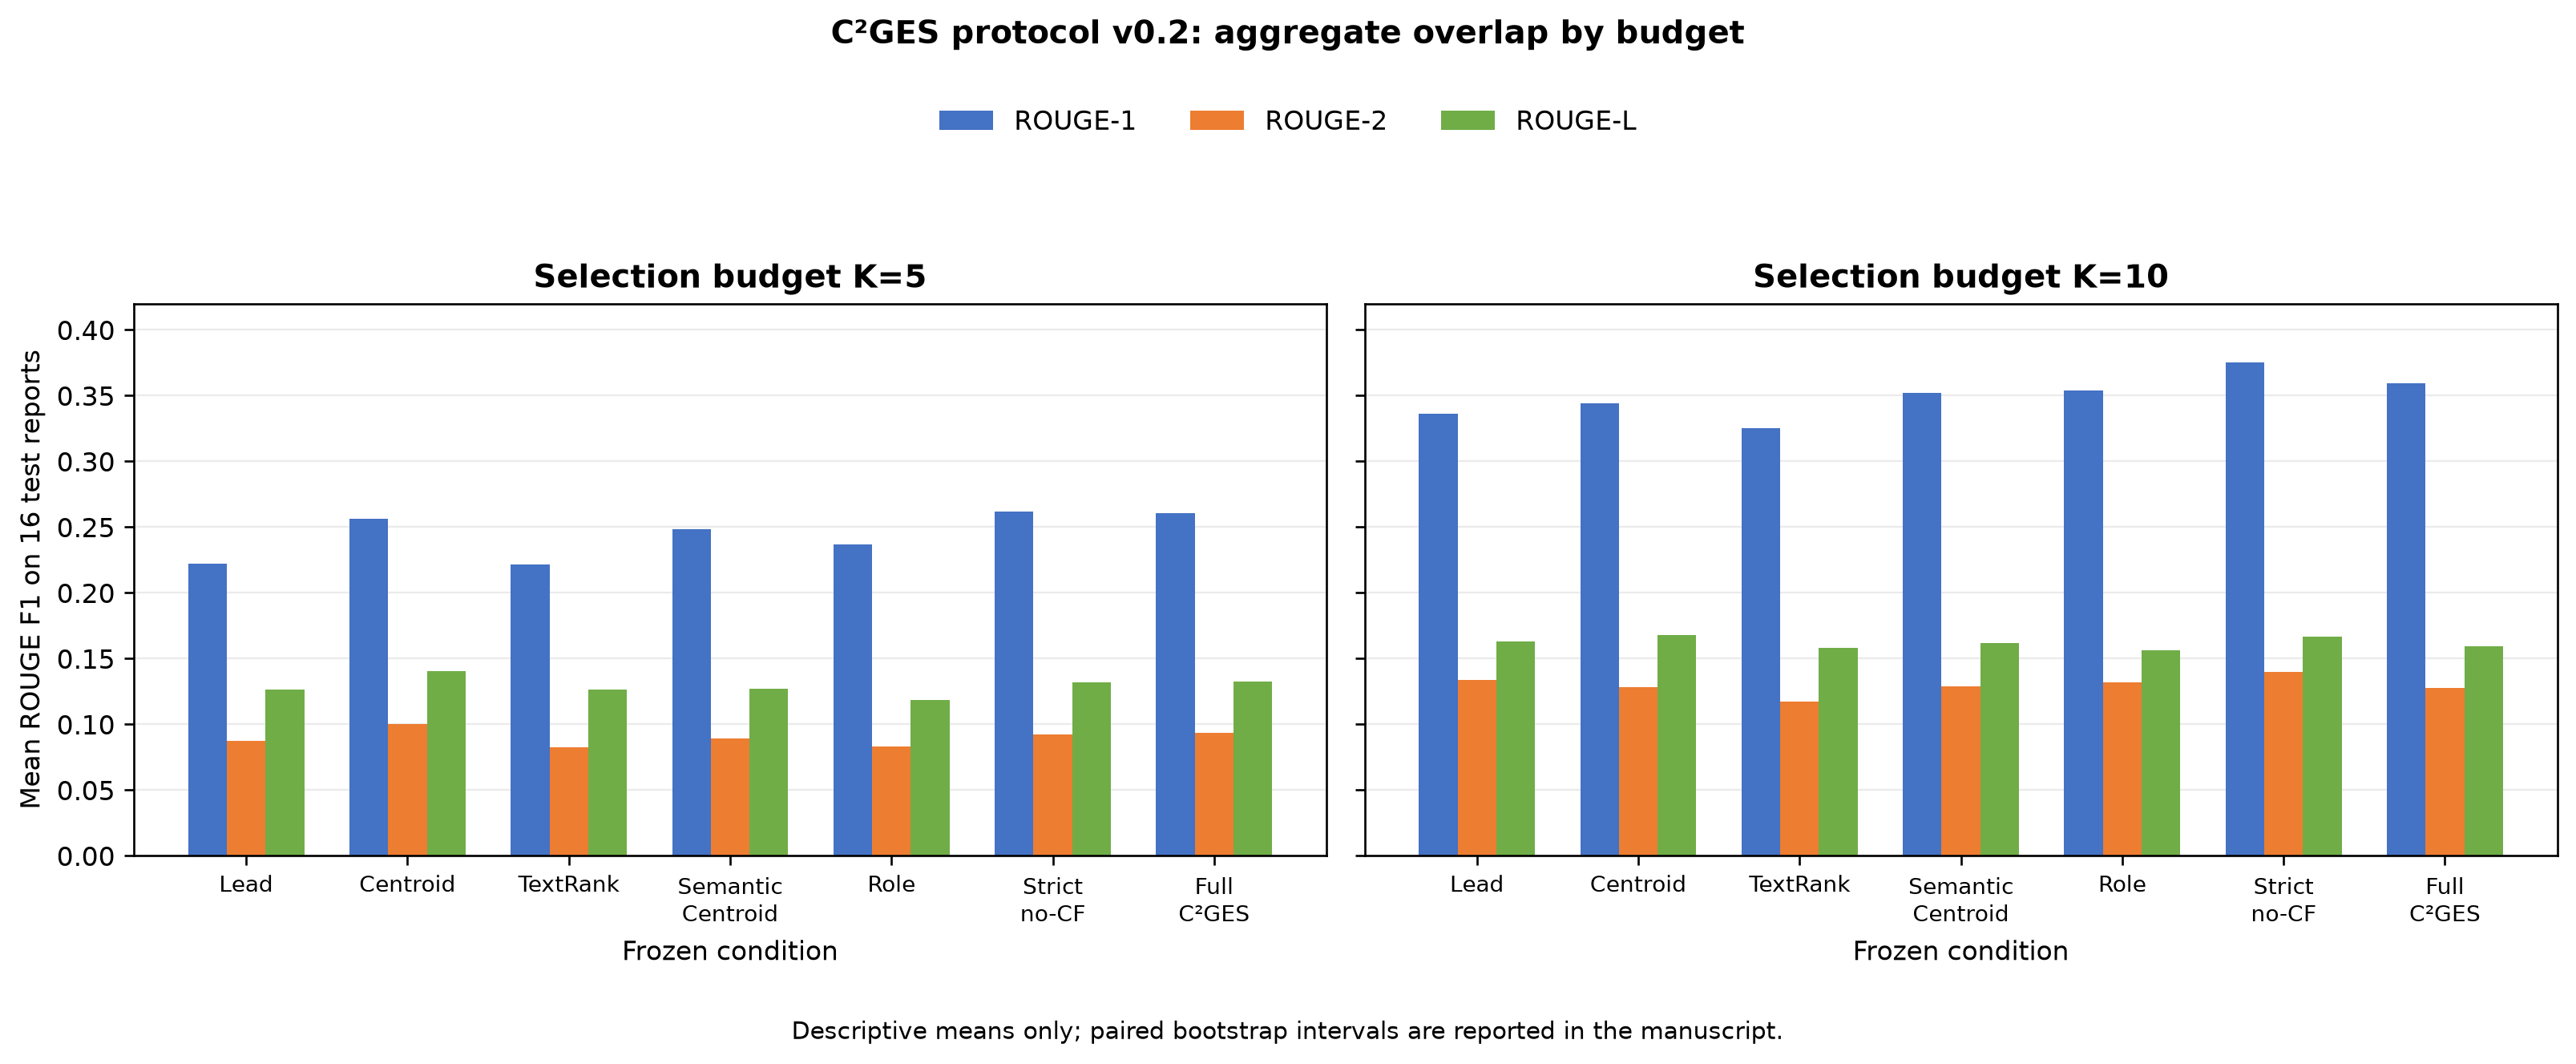
\includegraphics[width=\textwidth]{figures/fig_c2ges_v02_rouge_by_budget.png}
\caption{Mean test-set ROUGE F1 for seven frozen conditions at $K=5$ and $K=10$ (16 reports). Values are read directly from the protocol-v0.2 aggregate artifact. Bars show means, not uncertainty intervals; paired report-level bootstrap intervals are reported in the text.}
\label{fig:rouge-budgets}
\end{figure}

\begin{table}[H]
\caption{Budget sensitivity at $K=10$. Bold marks the observed column maximum only.}
\label{tab:k10}
\centering
\begin{tabular}{lrrrrr}
\toprule
Condition & R-1 F1 & R-2 F1 & R-L F1 & Silver coverage & Redundancy\\
\midrule
Lead & 0.3361 & 0.1337 & 0.1629 & 0.3000 & \textbf{0.0516}\\
Centroid & 0.3439 & 0.1281 & \textbf{0.1681} & 0.3625 & 0.1309\\
TextRank & 0.3252 & 0.1171 & 0.1583 & 0.2750 & 0.1376\\
Semantic Centroid & 0.3521 & 0.1288 & 0.1616 & 0.2750 & 0.0984\\
Role & 0.3540 & 0.1321 & 0.1565 & \textbf{0.6250} & 0.0585\\
Graph without CF (strict) & \textbf{0.3755} & \textbf{0.1396} & 0.1668 & 0.6125 & 0.0762\\
\cges{} Full & 0.3595 & 0.1276 & 0.1593 & 0.5625 & 0.0650\\
\bottomrule
\end{tabular}
\end{table}

The increase from $K=5$ to $K=10$ should not be interpreted as improved precision or causal validity. It primarily demonstrates the length sensitivity of ROUGE when official Executive Summaries have a median length of 790.5 words.

\subsection{Reproducibility}

Run~01 and a complete Run~02 in a new directory each produced 224 prediction rows (16 reports, 7 conditions, 2 budgets). The prediction, aggregate, and bootstrap files were byte-identical, with SHA-256 values \texttt{1f82961f...1e43be1}, \texttt{b26d436a...5c82f71}, and \texttt{4ca4aacd...54b5ab8}. All document--budget--condition cells were present, every extract contained unique sentence IDs up to its budget, and all metrics were finite values in $[0,1]$.

\subsection{Auxiliary Evidence-Selection Boundary}

The existing document-grouped FEVER study contains 8000 training, 1500 development, and 1500 test instances, drawn from 745, 141, and 145 underlying documents, respectively, with zero cross-split overlap. Across five downstream seeds, predicted-label evidence F1 was 0.4920 (SD 0.0021) at $K=3$, compared with 0.4864 for BM25. However, predicted-role minus label-blind was only +0.0010 with intervals crossing zero, and frozen MiniLM/BGE comparison families had no Holm-adjusted promoted finding. These assets verify a sentence-ranking workflow but do not establish domain summarization quality, a causal-role advantage, or the effectiveness of the present graph intervention.

\section{Discussion}

\subsection{Supported Interpretation}

The study establishes an end-to-end, offline, auditable report-summarization benchmark and method. Full \cges{} improves ROUGE-1 over Lead and TextRank at five sentences and selects less redundant extracts than both centroid baselines. No method dominates all overlap measures: lexical Centroid is strongest on observed ROUGE-L at both budgets, and strict no-CF is strongest on observed ROUGE-1 at both budgets and ROUGE-2 at ten sentences.

The counterfactual result is negative. A strict removal test is tied at five sentences, and the ten-sentence ROUGE-1 interval is unfavorable to Full. Therefore, the graph-flow sensitivity term cannot be presented as an effective innovation in its current form. Retaining and reporting this result is more informative than attributing the system-level ROUGE-1 contrast to the named component.

\subsection{Meaning of Causal and Counterfactual}

The typed graph is inspectable, but its relations are role-compatible textual proxies rather than verified physical causality. Interpretability means that nodes, edges, weights, interventions, scores, and sentence IDs can be audited. It does not mean the graph represents the true data-generating process or that selected sentences are correct outside their source context.

Likewise, removing a node measures graph-flow dependence. It does not answer how the grid would have behaved under an operational intervention. The retained title should therefore always be accompanied by this implementation boundary in the abstract, methods, and limitations.

\subsection{Practical Relevance}

The immediate output is a five- or ten-sentence source-ordered packet with stable identifiers and component audit information. It can accelerate navigation of a long reliability report, but it is not autonomous root-cause analysis. Operational use requires source links, human review, access controls, and a documented way to reject or supplement selections.

The benchmark contains genuine NERC reliability and disturbance documents, not utility-internal work orders. Generalization to confidential maintenance records requires a separate license, parsing audit, and sealed evaluation.

\subsection{Limitations and Next Gate}

The test set has only 16 reports. Report-level resampling respects the unit of analysis but cannot represent all grid-report genres. References are much longer than five- or ten-sentence predictions, and ROUGE does not measure engineering usefulness, factual sufficiency, or causal correctness.

Role evidence is machine silver and may influence selection; its coverage cannot serve as expert validation. A human domain study requires a frozen manual, multiple independent qualified reviewers, blinded labels, retained disagreements, human adjudication, and a sealed test set.

The graph uses lexical roles, token overlap, distance, and weighted degree. It has no trained GNN, T5 generator, structural causal model, or physical simulator. The local semantic baseline reduces but does not eliminate the need for stronger report summarizers. The 15 comparisons per budget are not multiplicity-adjusted.

Most importantly, no R1 test result may be used to tune the counterfactual term. R2 must first register a candidate CF family, weight search space, selection objective, and tie-breaking rule using only the 12 development reports. The chosen form must then be frozen before a single one-shot evaluation on the unchanged 16-report test set. If development-only selection yields no acceptable CF specification, R2 should retain the negative R1 result rather than search the test set.

PDF section parsing remains another risk. The retained failed boundary run shows why every future data revision requires a new directory, new hash, and regression tests instead of silent replacement.

\section{Conclusions}

The rebuilt \cges{} constructs a typed sentence-level causal proxy graph, performs deterministic leave-one-node-out graph intervention, and selects a source-ordered extract under causal-function coverage and redundancy constraints. The frozen public NERC benchmark contains 28 eligible reports and 16 test reports with official Executive Summaries as references.

At five sentences, Full reaches ROUGE-1/2/L F1 of 0.2608/0.0934/0.1323 and has positive ROUGE-1 intervals relative to Lead and TextRank. It does not lead on ROUGE-L, is unresolved relative to local Semantic Centroid, and obtains no benefit from the strict CF component. At ten sentences, strict no-CF has higher observed ROUGE scores, with a wholly negative unadjusted Full-minus-no-CF ROUGE-1 interval.

The supported contribution is an auditable benchmark, executable graph-constrained baseline, honest counterfactual ablation, and reproducible evidence ledger. Stronger causal claims require a development-only redesign followed by one frozen test evaluation, while domain-performance claims require independent expert evidence.

\supplementary{The reproducibility package contains the source manifest and exclusion audit, frozen v0.1 and v0.2 configurations, code and runtime hashes, local semantic-model revision and tree hash, unit tests, both completed v0.2 run directories, the 224-row prediction ledger, aggregate metrics, report-level bootstrap outputs, and assembly audit. Public source PDFs are not redistributed where third-party permissions do not allow it.}
\authorcontributions{Conceptualization, B.L. and Y.Y.; methodology, B.L.; software, B.L.; validation, B.L.; formal analysis, B.L.; investigation, B.L.; resources, Y.Y.; data curation, B.L.; writing---original draft preparation, B.L.; writing---review and editing, B.L. and Y.Y.; visualization, B.L.; supervision, Y.Y.; project administration, Y.Y.; funding acquisition, Y.Y. All authors have read and agreed to the published version of the manuscript.}
\funding{This research was funded by the Science and Technology Project of NARI Group Corporation (State Grid Electric Power Research Institute), grant number 521300250006.}
\institutionalreview{Not applicable. This study did not involve humans or animals; it uses public technical reports and an existing public human-annotated auxiliary benchmark.}
\informedconsent{Not applicable.}
\dataavailability{FEVER is available from its original providers \cite{thorne2018fever}. Public code and license-cleared reproducibility materials are available at \url{https://github.com/gaoxingkele/c2ges}. Owing to third-party licensing restrictions, NERC source documents and submission-version materials not included in the public repository are available from the corresponding author upon reasonable request for editorial and peer-review verification, subject to third-party permission and applicable licenses. The verification package includes source URLs and hashes, the frozen dataset manifest, builder and audit code, configurations, method implementation, predictions, statistics, and reproduction outputs.}
\acknowledgments{During preparation of this manuscript, AI-assisted tools were used for drafting, editing, code review, and reproducibility checks. The authors reviewed and edited all outputs and take responsibility for the publication. Machine-produced labels are not presented as human or domain-expert ground truth.}
\conflictsofinterest{The authors declare no conflicts of interest. The funder had no role in the design of the study; collection, analysis, or interpretation of data; writing of the manuscript; or decision to publish the results.}

\begin{adjustwidth}{-\extralength}{0cm}
\reftitle{References}
\bibliography{references_cited_verified}
\PublishersNote{}
\end{adjustwidth}
\end{document}
